\documentclass[letterpaper]{article}
\usepackage{aaai}
\usepackage{times}
\usepackage{helvet}
\usepackage{courier}
\usepackage{url}
\usepackage{graphicx}
\usepackage{tikz} % SW: Added for plots
\frenchspacing

%\usepackage[utf8]{inputenc} % allow utf-8 input -- cannot use with AAAI! A.S.
%\usepackage{hyperref}       % hyperlinks
\usepackage{url}            % simple URL typesetting
\usepackage{booktabs}       % professional-quality tables
\usepackage{amsfonts}       % blackboard math symbols
\usepackage{nicefrac}       % compact symbols for 1/2, etc.
\usepackage{microtype}      % microtypography
\usepackage{amssymb}
%\usepackage{natbib} % cannot use with AAAI! A.S.

\usepackage{amsthm} % The amsthm package provides extended theorem environments
\usepackage{float}
\usepackage{sgame, tikz} % Game theory packages
\usepackage{caption}
\usepackage{algorithm,algpseudocode}
\usepackage{makecell}
 \usepackage{multirow}
 \usepackage{graphicx}
\theoremstyle{definition}
\newtheorem{definition}{Definition}
\newtheorem{finding}{Finding}
\captionsetup{font=footnotesize}


% The \author macro works with any number of authors. There are two
% commands used to separate the names and addresses of multiple
% authors: \And and \AND.
%
% Using \And between authors leaves it to LaTeX to determine where to
% break the lines. Using \AND forces a line break at that point. So,
% if LaTeX puts 3 of 4 authors names on the first line, and the last
% on the second line, try using \AND instead of \And before the third
% author name.


% Alex' macro
\usepackage{xspace}
\newcommand{\OMIT}[1]{}
\newcommand{\xhdr}[1]{\vspace{1mm} \noindent{\bf #1}}
\newcommand{\ie}{{\em i.e.,~\xspace}}
\newcommand{\eg}{{\em e.g.,~\xspace}}
\newcommand{\TS}{\mathrm{TS}}
\newcommand{\DEG}{\mathrm{DEG}}

% a very useful package for edits and comments, from David Kempe (USC)
\usepackage{color-edits}
%\usepackage[suppress]{color-edits}  % use this to suppress the package
\addauthor{as}{red}    % as for Alex
\addauthor{ga}{blue}  % ga for Guy
\addauthor{sw}{orange} % sw for Steven
% e.g. for Alex, provides \asedit{}, \ascomment{} and \asdelete{}.


\begin{document}

%\title{Learning and Reputation under Monopoly and Duopoly: \\A Competing Bandits Approach}

%\title{Competing Bandits: Exploration and Competition under Duopoly}

\title{Competing Bandits: The Perils of Exploration under Competition}


%\author{Guy Aridor\textsuperscript{1}, Kevin Liu\textsuperscript{2}, Aleksandrs Slivkins\textsuperscript{3},
%Zhiwei Steven Wu\textsuperscript{4} \\
%{\textsuperscript{1}Columbia University, Department of Economics}\\
%{\textsuperscript{2}Columbia University, Department of Computer Science}\\
%{\textsuperscript{3}Microsoft Research, New York, NY}\\
%{\textsuperscript{4}University of Minnesota - Twin Cities, Department of Computer Science}
%}
\maketitle


\begin{abstract}
We empirically study the interplay between \textit{exploration} and \textit{competition}. Systems that learn from interactions with users
often engage in \emph{exploration}: making potentially suboptimal decisions in order to acquire new information for future decisions. However, exploration may hurt system's reputation in the near term, with adverse competitive effects. In particular, a system may enter a ``death spiral" when decreasing market share leaves the system with less users to learn from, which degrades system's performance relative to competition and further decreases the market share.

We ask whether better exploration algorithms are incentivized under competition. We run extensive numerical experiments in a stylized duopoly model in which two firms deploy multi-armed bandit algorithms and compete for myopic users.  We find that duopoly \asedit{and monopoly} tend to favor a primitive ``greedy algorithm" that does not explore, whereas a temporary monopoly (a duopoly with an early entrant) may incentivize better bandit algorithms. Our findings provide new intuition on the ``first-mover advantage" in the digital economy.
\end{abstract}


\OMIT{ %%% Guy's original abstract
\begin{abstract}
We empirically study the interplay between \textit{exploration} and \textit{competition} - how platforms that learn from interactions with users tradeoff between making potentially suboptimal choices in order to acquire new information and the reputational consequences of this exploration which potentially has adverse competitive effects. Our model considers competition for myopic users between two firms deploying multi-armed bandit algorithms that face the same underlying multi-armed bandit instance. The users select between the firms according to a reputation score, which is a function of the rewards past users have experienced from this firm.

We ask whether better algorithms are incentivized under varying degrees of competition. The environments we consider are a monopoly, a duopoly with one firm serving as an early entrant (a temporary monopoly), and a duopoly. We show that, under certain conditions, monopoly and duopoly do not incentivize the adoption of better learning algorithms due to the reputational costs of exploration, but that a temporary monopoly may incentivize the adoption of better learning algorithms. Additionally, we interpret our results as providing an alternative intuition behind the classic first-mover advantage which gives the incumbent firm both a data advantage and a reputational advantange. Finally, we ask whether in this setting the data advantage or the reputational advantage of the early entrant serves as stronger barriers to entry.
\end{abstract}
} %%%%%%%

\section{Introduction}\label{section:1}

Many modern online platforms simultaneously compete for users as well as learn from the users they manage to attract. This creates a tradeoff between \textit{exploration} and \textit{competition}: firms experiment with potentially sub-optimal options for the sake of gaining information to make better decisions tomorrow, while they need to incentivize consumers to select them over their competitors today. For instance, Google Search and Bing compete for users in the search engine market yet at the same time need to experiment with their search and ranking algorithms to learn what works best.

Platforms routinely deploy \asedit{A/B tests}, and are increasingly adopting  more sophisticated exploration methodologies based on \emph{multi-armed bandits}, a well-known framework for exploration and making decisions under uncertainty. While deploying ``better" learning algorithms for exploration would improve performance, this is not necessarily beneficial under competition, \asedit{even putting aside the deployment/maintenance costs}. In particular, excessive experimentation may hurt platform's reputation and decrease market share in the near term. This would leave the learning algorithms with less users to learn from, which may further degrade platform's performance relative to competitors who keep learning and improving from \emph{their} users, and so forth.

We ask whether competition incentivizes adoption of "better" algorithms for exploration. We investigate this issue via extensive numerical experiments in a stylized duopoly model. In our model, two firms compete for users, and simultaneously learn from them. Each firm commits to a multi-armed bandit algorithm, and \emph{explores} according to this algorithm. Users select between the two firms based on the current reputation score: rewards from the firm's algorithm, averaged over a recent time window. \asedit{Each firm's objective} is to maximize its market share ---the fraction of users coming to them.

\tikzstyle{level 1}=[level distance=3.5cm, sibling distance=4.0cm]
\tikzstyle{level 2}=[level distance=3.5cm, sibling distance=2cm]
\tikzstyle{below} = [align=center]

\begin{figure}
\begin{center}
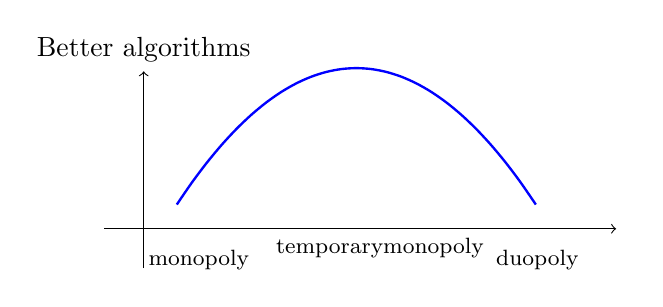
\begin{tikzpicture}
      \draw[->] (-.5,0) -- (6,0) node[right] {};
      \draw[->] (0,-.5) -- (0,2) node[above] {Better algorithms};
      \draw[scale=0.6,domain=0.7:8.3,smooth,variable=\x,blue, line width=0.3mm] plot ({\x},{3.4 - 0.2 * (\x - 4.5)^2});
     \node[below] at (0.7, -0.15) {\footnotesize monopoly};
     \node[below] at (3, 0) {\footnotesize temporary \\ monopoly};
     \node[below] at (5, -0.15) {\footnotesize duopoly};
 \end{tikzpicture}
 \caption{A stylized ``inverted-U relationship" between strength of competition and ``level of innovation".}
\label{fig:inverted-U}
\end{center}
\end{figure}

We consider varying levels of competition, from monopoly to \emph{temporary monopoly} (a duopoly with an early entrant), to a true duopoly in which both firms start at the same time. We find that a ``greedy algorithm" that does not explicitly explore is most beneficial under duopoly. This algorithm also prevails under monopoly, simply because it tends to be easier to deploy. Whereas a temporary monopoly incentivizes more advanced exploration algorithms that perform better in the long run. The disincentives to explore under duopoly arise entirely because of ``reputational costs", rather than R\&D costs (which are absent from our model).


\asedit{Interpreting the adoption of better algorithms as ``innovation", our findings can be framed in terms of an ``inverted-U relationship" between competition and innovation (see Figure~\ref{fig:inverted-U}). This relationship -- too little or too much competition is bad for innovation, but intermediate levels of competition tend to be better -- is a familiar theme in the economics literature, dating back to \cite{Schumpeter-42}.}



Our findings on temporary monopoly shed light on the ``first-mover advantage" phenomenon in the digital economy. In this scenario, the incumbent firm enjoys both a ``data advantage" and a ``reputational advantange". We further investigate which of the two is a stronger barrier to entry. \ascomment{and find what? and what's the new intuition?}









\subsection{Discussion and related work}
Our work is related to a longstanding economics literature on competition vs. innovation, \eg \cite{Schumpeter-42,barro2004economic,Aghion-QJE05}. While this literature focuses on R\&D costs of innovation, ``reputational costs" thereof seem new and specific to exploration.

Multi-armed bandits (MAB) is a tractable abstraction for the tradeoff between exploration and \emph{exploitation} (making good near-term decisions based on available information). MAB problems have been studied for many decades, see \cite{Bubeck-survey12} for background. We consider a simple and well-understood MAB model with i.i.d. rewards \cite{bandits-ucb1}. We focus on a well-known distinction between the ``greedy" (exploitation-only) algorithm, "naive" MAB  algorithms that separate exploration and exploitation, and better MAB algorithms that combine the two. As a token example of ``near-optimal" bandit algorithms, 
we use a classic algorithm called ``Thompson Sampling", see \cite{TS-survey-FTML18} for background.

The study of competition vs. exploration has been initiated in \cite{CompetingBandits-itcs16}. Their model differs from ours in two key respects. First, users do not see any signal about firms' past performance, and instead choose between firms according to the Bayesian-expected reward. Second, they vary the strength of competition using assumptions about (ir)rational consumer behavior, whereas we use early entry. Their results are purely theoretical; their model is amenable to proofs but not to numerical experiments.

The interplay between exploration, exploitation and incentives has been studied in other scenarios: incentivizing exploration in a recommendation system,
    \eg \cite{Kremer-JPE14,Frazier-ec14,Che-13,ICexploration-ec15,Bimpikis-exploration-ms17},
dynamic auctions
    (see \cite{DynAuctions-survey10} for background),
online ad auctions, \eg
    \cite{MechMAB-ec09,DevanurK09,NSV08,Transform-ec10-jacm,Amin-auctions-nips13},
and human computation
    \cite{RepeatedPA-ec14,Ghosh-itcs13,Krause-www13}.

\OMIT{ %%%%%%
The interplay between exploration, exploitation, and incentives has been studied in several other settings, the most relevant to this paper being \cite{che2017recommender}, \cite{kremer2014implementing}, \cite{mansour2015bayesian}. The strategic experimentation literature in economics, such as \cite{bolton1999strategic} and \cite{keller2005strategic}, studies models with self-interested agents jointly performing exploration whereas in this paper the firms cannot observe the actions or the payoffs of the other firms and exploration is coordinated by the consumers.
} %%%%%%%%

Our setting is also closely related to the "dueling algorithms" framework \cite{DuelingAlgs-stoc11}, but this framework considers offline / full feedback scenarios whereas we focus on online machine learning problems.


\section{Model}\label{sec:model}

\textbf{Overview} There are two firms and $T+2k$ agents where $k$ is the warm start, or the agents that each firm gets for free at the beginning of the game and $T$ is the number of rounds in the game. The timing of events is as follows:
\begin{enumerate}
\item At $t = 0$, the firms simultaneously commit to following a learning algorithm from a set of algorithms $\mathcal{A}$
\item Still at $t = 0$ we suppose that each firm gets $k$ agents as a ``warm" start. The algorithm that the firm commits to makes $k$ rounds of progress and uses this information to initialize its information set. Additionally, the reputation score used by the agents is initialized using the rewards from these $k$ rounds.
\item A new agent arrives each round (and lives for only one round), starting at $t = 1$, and chooses the firm with the higher reputation at the time.
\item The firm that is chosen selects an action $a_{t} \in A$ from a set of actions that is fixed across firms and rounds.
\item Both the agent and the firm observe the reward $r_t \in [0, 1]$ from the action. The agent reports this reward to the firm and the future agents and the reputation score for the chosen firm is updated.
\item Repeat 2-4 for $T$ rounds.
\end{enumerate}

Generally, the rewards are independent and identically distributed with a common prior.  For computational tractability we restrict our focus to Bernoulli-distributed rewards with Beta priors. Each firm faces a multi-armed bandit problem with no initial information \footnote{For algorithms that require a prior to operate, such as Thompson Sampling, we use a "fake" prior of $Beta(\alpha=1,\beta=1)$}. We assume that the firms commit to a multi-armed bandit learning algorithm at the start of the world and that there are no informational spillovers from their competitors so that they can only learn from the agents that select them.\swcomment{this seems misleading and should not be here. just say that each action has bernouli rewards with unknown means}

\noindent \textbf{Agents} We suppose that agents are homogenous, myopic, and non-strategic. The utility function for the agents is simply to maximize their reward in the one period in which they are alive. We suppose that agents do not attempt to manipulate the strategy of the firm, do not take the strategies of the firm into account when choosing between the firms, and do not condition their behavior on calendar time. In our model, each agent uses the average reward of past agents as a proxy for their expected utility. For simplicity, the reputation score, $R_{jt}$ is defined as a sliding window average\footnote{Another natural formulation would be to have exponential discounting of the past rewards. We believe that the results should be qualitatively similar to those presented here as in both formulations the more recent past matters more than the distant past.}.
\begin{center}
$R_{jt} = \frac{1}{M} \sum\limits_{i=1}^{M} r_{t_j-i}$
\end{center}

Note $t_j$ is the \textit{local} time of the firm, not the global time, so the reputation score is the sliding window average of the last $M$ times that firm $j$ was selected by the agents.\swcomment{define ``calendar time'' and ``local time'' formally... don't think the current reputation defn makes sense} The warm start of $k$ rounds allows this reputation score to be well-defined once the "competition game" begins. In our model the agents deterministically choose the firm with the higher reputation score and ties are broken uniformly at random.

\noindent \textbf{Firms} We suppose that the firms simply care about maximizing their expected market share (i.e. maximizing the number of $T$ agents who select them). We model the "competition game" between firms as a simultaneous move game where both firms commit to a learning algorithm at $t = 0$.

\noindent \textbf{MAB algorithms} We suppose that firms commit to a learning algorithm from a fixed set of algorithms $\mathcal{A}$. We partition the set of possible learning algorithms into three different types of learning algorithms and restrict $\mathcal{A}$ to contain a representative each algorithm from each class:
\begin{enumerate}
\item "Smart" algorithms that engage in adaptive exploration and combine exploration and exploitation. We consider Thompson Sampling (from hereon $\TS$) from this class, which, in a given period, will pull an arm according to the probability that that arm is "optimal" in the sense of having the highest mean reward %\cite{Shipra-colt12}.
\item "Naive" algorithms that engage in non-adaptive exploration algorithms and separate exploration and exploitation. We consider $Dynamic$ $\epsilon$-$greedy$ (from hereon $\DEG$) from this class, which, in a given period, pulls the arms with the highest posterior mean for $1 - \epsilon$ probability and selects a random arm with $\epsilon$ probability. For our experiments we keep $\epsilon = 0.05$ fixed.
\item Greedy / myopic algorithms that engage in no purposeful exploration and take the best short-sighted action. We consider $DynamicGreedy$ (from hereon $DG$) from this class, which, in a given period, pulls the arm with the highest posterior mean.
\end{enumerate}

In the standard multi-armed bandit problem it is known that $\TS > \DEG > DG$ in terms of maximizing cumulative reward over a sufficiently large time horizon. The primary question that we want to understand is when, in competition, are the firms incentivized to adopt the "better" algorithms?

\noindent \textbf{Incumbent} In some of our experiments we modify our model so that one firm enters the market $X$ number of rounds before the other. We refer to the firm that enters before as the "incumbent" and the firm that enters after $X$ rounds as the "entrant." In the $X$ rounds before the "entrant" enters the incumbent is a temporary monopolist as the agents that arrive in these $X$ rounds are forced to select the incumbent since it is the only firm in the market and there is no outside option. We treat $X$ as being an exogenous element of the model and study the consequences for a fixed $X$. We have that both the incumbent and entrant commit to a learning algorithm \textit{before} either firm receives any agent. After the $X$ rounds, both firms still receive the $k$ warm start agents.

\section{Simulation Details}\label{section:3}

We evaluate the consequences of our model via simulation.\swcomment{In the process of removing ``prior'' throughout}

\textbf{Bandit Instances} We look at bandit instances drawn from three different bandit \swedit{distributions} that capture different types of learning problems. Recall that we only consider Bernoulli rewards, which are fully parameterized by the means. For these experiments we fix the number of arms we consider, $K = 10$.
\begin{enumerate}
\item Needle In Haystack - $K-1$ arms with mean 0.5 and 1 arm with 0.7.
\item Uniform - the $K$ arms have means drawn uniformly at random from $[0.25, 0.75]$
\item "Heavy Tail" - the $K$ arms have means drawn from $Beta(\alpha=0.6, \beta = 0.6)$. With this prior it was likely to have means at the "extremes" or means that were close to 0 as well as means that were close to 1.
\end{enumerate}

\noindent \textbf{Simulation of Competition Game} Unless otherwise noted, all of the reported results utilize the same set of randomly drawn bandit instances and realizations from the prior. Namely, for each bandit prior we draw $N = 1000$ bandit instances. For each of these instances we run simulations of our model for varying values of $k$ and $X$. We take the maximum values of $k$ and $X$ for the simulations we run, $k_{max}$ and $X_{max}$ respectively, and compute a realization table of dimension $(T+k_{max}+X_{max}) \times K$.

This realization table, as well as fixing the random seed for the same bandit instance and realization table across experiments, ensures that differences in algorithm performance are not due to noise in the realizations but due to differences in the algorithms in the different experimental settings. In the competition game we draw from the $T \times K$ portion of the table, so that if two different algorithms picks arm $a$ at time $t$, they get the same $[a, t]$ realization in the table. This setup also ensures that in the warm start period, increasing the warm start from $k$ to $k + 10$ results in the same behavior in the first $k$ rounds.

For the simulations we fix the sliding window size $M = 100$. Low values of $M$ induced too much random noise into the results and we found that increasing $M$ to be larger than $100$ did not make a substantial qualitative difference so we fix this value.

\section{Performance in Isolation}\label{section:4}

We evaluate the performance of the different learning algorithms on the bandit priors we consider in isolation. There are two reasons why this is important to consider. First, we want to confirm that the reputation ordering of the algorithms is what we would expect according to the multi-armed bandit literature where, according to the mean reputation, $\TS > \DEG > DG$ for sufficiently large $t$. Second, we want to better understand what statistics of the priors we can look at in isolation in order to help us predict and understand what to expect in the competition game.

\begin{figure}
\caption{Mean Reputation Trajectories in Isolation}
\includegraphics[scale=0.35]{"figures/nih_iso_mean"}
\label{prelim_means}
\caption*{\tiny{The plots contain the average reputation over $1000$ runs for a memory size of $100$ where, for a given $t$, we record the reputation of a given algorithm on a given instance and then average this value across all the runs. The shaded area display 95\% confidence intervals.}}
\end{figure}

Figure \ref{prelim_means} shows that the mean reputation ordering is as we would expect for the Needle In Haystack prior \footnote{The mean reputation ordering that we expect also holds for the other two priors and the results for those can be found in the supplementary material.}.

\begin{figure}[H]
\caption{Reputation Distribution}
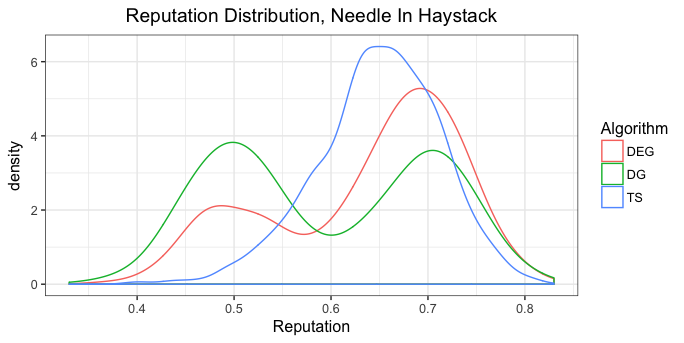
\includegraphics[scale=0.35]{figures/rep_distribution_nih}
\label{rep_dist_nih}
\caption*{\tiny{The plots contain a kernel density estimate of the reputation distribution at $t = 500$}}
\end{figure}

\begin{finding}
\textit{The mean performance of an algorithm is not a sufficient statistic for understanding the performance of an algorithm in competition. Looking at the distribution of reputation difference between algorithms we find that it tend is skewed to the right. Additionally we provide a counterexample where the mean performance does not predict the result of the competition game.}
\end{finding}


Is looking at the mean performance of between two algorithms sufficient for understanding what happens in competition? To answer this, we first look at the entire reputation distribution at $t = 500$ in Figure \ref{rep_dist_nih}. We see that the ``naive" algorithms $DG$ and $\DEG$ have a bi-modal reputation distribution whereas $\TS$ does not. The intuition for this is that, for Needle In Haystack, $DG$ either finds the best arm or not. If it does, then since it engages in no purposeful exploration it will do better than any algorithm that engages in purposeful exploration over sufficiently many rounds. However, if it does not then it will get stuck on a bad arm and lose to $\TS$ or $\DEG$. In these cases its reputation may be substantially worse but for the competition game the relative comparison between them is all that matters \footnote{This holds for our model and the decision rule of the agents, though the absolute difference may matter if, for instance, we consider the SoftMax decision rule in \cite{CompetingBandits-itcs16}}.

To better capture the comparison between two algorithms we explicitly plot the distribution of the reputation difference between $\TS$ and $DG$. This figure seems to confirm the intuition noted previously since the reputation distribution has its largest mass around the point just below 0 but it is skewed to the right even as $t$ gets large. Given the skewedness of the distribution, the mean is not a representative statistic of the entire reputation difference distribution. There are alternative statistics that we could consider such as the median or numerically calculating $\Pr(reputation(TS) - reputation(DG)) > 0$ using the estimated density, but instead we define a simple and natural statistic to help us reason about what happens under competition, the \textit{relative reputation proportion}.

\begin{figure}[H]
\caption{Reputation Difference Distribution}
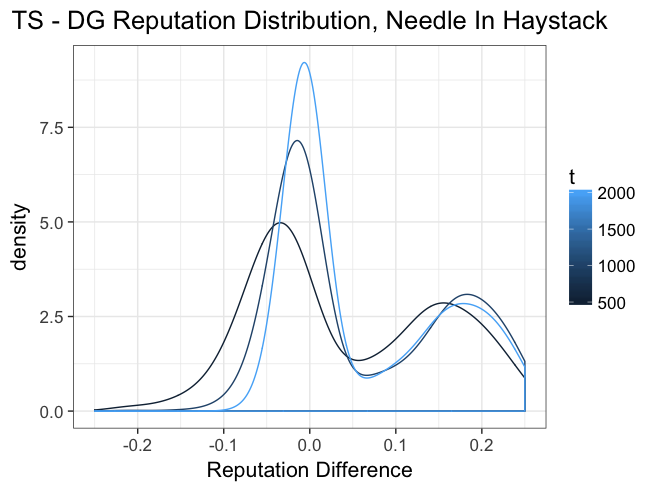
\includegraphics[scale=0.35]{figures/ts_dg_rep_diff_nih}
\label{ts_dg_rep_diff_nih}
\caption*{\tiny{The plots contain a kernel density estimate of the difference in reputation between $\TS$ and $DG$ across $t$}}
\end{figure}

\begin{definition}
\textit{Relative Reputation Proportion} - the proportion of simulations in which algorithm $A$ had at least as high of a reputation as algorithm $B$ for a fixed time $t$
\end{definition}


\begin{finding}
\textit{Purposeful exploration can lead to relative reputational costs compared to the greedy alternative and this leads to $\TS$ doing worse than $DG$ for small time horizons. We observe this under the Uniform and Heavy Tail priors. However, it is not observed under the Needle In Haystack prior}
\end{finding}

The relative reputation statistic corresponds to running the bandit algorithms in isolation on the same instance and with the same realizations for $t$ rounds and then calculating the fraction of simulations at which an agent would select a firm playing $A$ over a firm playing $B$ at time $t$ \footnote{As further motivation for this statistic, one may be interested in if there is ever a case where, for sufficiently large $t$, we observe that $\DEG >DG$ or $\TS > DG$ according to the mean reputation but $DG > \DEG$ or $DG > TS$ according to the relative reputation proportion. In the supplementary material we have results showing that, for Heavy Tail prior with $K=3$ we have that $\DEG > DG$ according to the mean reputation but $DG > \DEG$ according to the relative reputation proportion. Additionally, these results carry over to the competition game}.

\begin{figure}[ht]
\caption{Relative Reputation Plots}
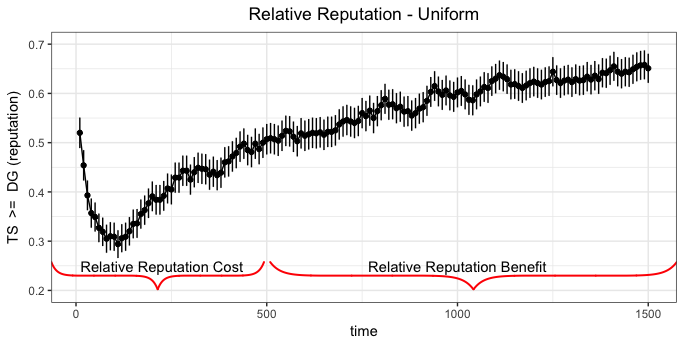
\includegraphics[scale=0.35]{figures/relative_uniform_annotated_plot}
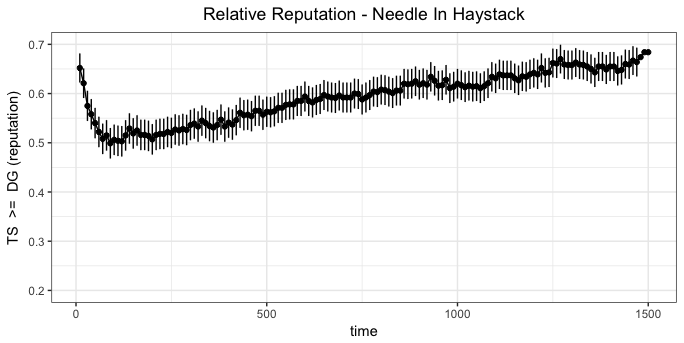
\includegraphics[scale=0.35]{figures/ts_dg_nih_10_prelim}
\caption*{\tiny{The plots contain the average reputation over $1000$ runs for a memory size of $100$ where, for a given $t$, we record the reputation of both of the algorithms on a given instance and then calculate the proportion of runs where $\TS \geq DG$. The shaded area display 95\% confidence intervals.}}
\label{relative_rep_plots}

\end{figure}



Figure \ref{relative_rep_plots} shows plots of the relative reputation proportion for $\TS$ vs $DG$ on the Uniform and Needle In Haystack prior. For the Uniform prior we see that, in the early rounds, $DG > TS$ for the majority of the simulations but that, eventually, $\TS > DG$. The intuition behind this is that, especially since the firms start with no substantive initial information, $\TS$ does purposeful exploration in the early rounds in order to acquire information. However, eventually the information acquired from purposeful exploration in the early rounds allows $\TS$ to make better decisions and achieve a higher reputation, especially when the instance is ``hard enough" so that $DG$ cannot trivially find the best arm. The early exploration leads to what we define as a \textit{relative reputation cost} and the eventual gain in reputation leads to what we define as a \textit{relative reputation benefit}.



\begin{definition}
\textit{Relative reputation cost and benefit} - the relative reputation loss an algorithm incurs from purposeful exploration compared to the greedy alternative. Here we treat it as an empirical definition based on the relative reputation proportion where the ``cost" regime is when the proportion $< 0.5$ and the ``benefit" regime is when the proportion is $> 0.5$ for the better algorithm. We call the priors where there is an early costly period followed by a later benefit period relative reputation costly priors.
\end{definition}
Is exploration always costly? Figure \ref{relative_rep_plots} also shows that for the Needle In Haystack prior, $\TS$ always does relatively better than $DG$. There are two contributing factors to this. First, $\TS$ identifies the best arm faster in the Needle In Haystack prior than the Uniform prior so that there is a shorter time horizon where $\TS$ needs to engage in purposeful exploration. Second, in the Needle In Haystack prior there are no ``bad" arms as there may be in the Uniform prior since by construction all the arms except one in Needle In Haystack are the same. Thus, when $\TS$ pulls a sub-optimal arm relative to its current information, the expected reward is the same as the greedy option that has not identified the best arm. However, with the Uniform prior, it is possible that the sub-optimal arm that is pulled has substantially lower expected reward relative to the greedy option. Thus, only the Uniform and Heavy Tail priors are relative reputation costly priors.

\section{Competition vs Better Algorithms: Inverted-U}\label{section:5}

In this section we document our main results that can be summarized via the empirically documented inverted-U relationship between competition and innovation described in \cite{Aghion-QJE05}. We consider three separate settings for our model: permanent monopoly, temporary monopoly (incumbent vs entrant), and permanent duopoly.

\begin{finding}
\textit{Under the priors that are relative reputation costly and with low warm start, the optimal strategies in the competition game are:
\begin{center}
\textbf{Permanent Monopoly} - $DG$ \\
\textbf{Temporary Monopoly} - $\TS$ \\
\textbf{Permanent Duopoly} - $DG$ \\
\end{center}
The conditions on $\TS$ being dominant under the temporary monopoly are that the incumbent is a temporary monopoly for sufficiently many periods.
}
\end{finding}

We interpret the move from permanent monopoly to temporary monopoly and temporary monopoly to permanent duopoly as increases in competition. We believe this is reasonable and consistent with the empirical results which define increases in competition as increases in a measure of market power (1 - the Lerner Index). In our model we have no prices and no costs and so we interpret increases in "market power" as decreases in the number of rounds where a firm has to compete for agents.

We utilize the same instances and realizations as in the section 4 and simulate the model described in section 2. We initially take the strategies of the firms as exogenous (chosen from $\mathcal{A}$) and simulate the model given these strategies in order to determine the expected payoffs associated with each pair of algorithms. Unless otherwise noted, all the results are reported at $t = 2000$.

\textbf{Permanent Monopoly} Under permanent monopoly only a single firm exists in the market for every period. Since, in our formulation, the firm only gets utility from a larger market share it is indifferent between each algorithm in $\mathcal{A}$ since, regardless of the algorithm it deploys, it will get the entire market. If we suppose that deploying the "better" algorithms has even an $\epsilon > 0$ cost, then the firm would choose to deploy $DG$.

\textbf{Permanent Duopoly} Permanent duopoly corresponds to the model described in section 2 where $X = 0$ so that both firms enter the market simultaneously. What algorithms are firms incentivized to deploy? We report the average market share taken over the $N$ simulations for a set of exogenous values of $k$. Additionally, we report the mean and median of an additional quantity which we define as the effective end of game.

\begin{definition}
\textit{Effective End of Game (EEOG)} - the last round, $t$, in a simulation where the agent alive at $t-1$ and the agent alive at $t$ choose different firms.
\end{definition}

Since both firms enter at the same time the game is symmetric and we only need to compute the payoffs of three pairs of strategies. We do not report them in the figures, but when both firms play the same algorithm the expected market share is 50/50.

\begin{finding}
\textit{For low warm starts, when exploration is relative reputation costly $DG >TS$ in competition, whereas when exploration is not relative reputation costly $\TS > DG$. For sufficiently large warm starts, $\TS$ is dominant across all priors.}
\end{finding}

Table \ref{sim_unif} shows the results under the Uniform prior. For the low values of the warm start we can see that $DG > TS$, but that for larger warm starts, $\TS > DG$ \footnote{The same results hold for the Heavy Tail prior and are reported in the supplemental material}. Looking at the relative reputation plots in Figure \ref{relative_rep_plots}, we can interpret fixing a warm start $k$ as fixing the starting point on the relative reputation plots. The proportion of first rounds in the competition game that will go to a firm playing alg $A$ over a firm playing alg $B$ will correspond to the relative reputation proportion at time $k$. The intuition for the result in competition aligns with the fact that, for Uniform and Heavy Tail, $\TS$ is relative reputation costly compared to $DG$ and so, for low warm starts, $\TS$ has not yet recovered from the relative reputation loss due to purposeful exploration and so $DG$ beats $\TS$. However, if we move the warm start sufficiently high so that $\TS$ moves to the relative reputation benefit regime, $\TS > DG$.

However, we do not always see that $DG > TS$ under some warm starts. Table \ref{sim_nih} shows the results for the Needle In Haystack prior where we see that $\TS > DG$. This is precisely due to the fact that, under the Needle In Haystack, $\TS$ is not relative reputation costly compared to $DG$ and thus we see that $\TS > DG$.


Combining these results with the fact that the EEOG values are relatively low across all warm starts \footnote{Interestingly, the EEOG also appears to be skewed to the right, similar to the distribution of reputation differences}, these observations seem to imply that understanding the performance of different algorithms in competition it is important to look at their performance for relatively small samples instead of asymptotically.

% latex table generated in R 3.4.0 by xtable 1.8-2 package
% Thu Aug 16 13:13:01 2018
\begin{table}[ht]
\centering
\caption{Duopoly Experiment Uniform}
\begin{tabular}{rlll}
  \hline
 & k = 20 & k = 250 & k = 500 \\
  \hline
TS vs DG & \makecell{\textbf{0.46} $\pm$0.03\\ eeog \\ avg: 230\\ med: 0} & \makecell{\textbf{0.52} $\pm$0.02\\ eeog \\ avg: 800\\ med: 754} & \makecell{\textbf{0.6} $\pm$0.02\\ eeog \\ avg: 910\\ med: 906.5} \\
  TS vs DEG & \makecell{\textbf{0.41} $\pm$0.03\\ eeog \\ avg: 180\\ med: 0} & \makecell{\textbf{0.51} $\pm$0.02\\ eeog \\ avg: 810\\ med: 734} & \makecell{\textbf{0.55} $\pm$0.02\\ eeog \\ avg: 970\\ med: 987} \\
  DG vs DEG & \makecell{\textbf{0.51} $\pm$0.03\\ eeog \\ avg: 470\\ med: 57.5} & \makecell{\textbf{0.48} $\pm$0.02\\ eeog \\ avg: 1000\\ med: 1088} & \makecell{\textbf{0.45} $\pm$0.02\\ eeog \\ avg: 1000\\ med: 1142} \\
   \hline
\end{tabular}
\label{sim_unif}
\end{table}

\begin{table}[ht]
\centering
\caption{Duopoly Experiment Needle In Haystack}
\begin{tabular}{rlll}
  \hline
 & k = 20 & k = 250 & k = 500 \\
  \hline
TS vs DG & \makecell{\textbf{0.64} $\pm$0.03\\ eeog \\ avg: 200\\ med: 27} & \makecell{\textbf{0.6} $\pm$0.03\\ eeog \\ avg: 370\\ med: 0} & \makecell{\textbf{0.64} $\pm$0.03\\ eeog \\ avg: 580\\ med: 121.5} \\
  TS vs DEG & \makecell{\textbf{0.57} $\pm$0.03\\ eeog \\ avg: 150\\ med: 14} & \makecell{\textbf{0.52} $\pm$0.03\\ eeog \\ avg: 460\\ med: 78.5} & \makecell{\textbf{0.56} $\pm$0.02\\ eeog \\ avg: 740\\ med: 627.5} \\
  DG vs DEG & \makecell{\textbf{0.46} $\pm$0.03\\ eeog \\ avg: 340\\ med: 128.5} & \makecell{\textbf{0.42} $\pm$0.02\\ eeog \\ avg: 650\\ med: 408} & \makecell{\textbf{0.42} $\pm$0.02\\ eeog \\ avg: 690\\ med: 466.5} \\
   \hline
\end{tabular}
\label{sim_nih}
\caption*{\tiny{The first line in each cell contains the average market share received by the firm playing Alg 1 (and the market share of Alg 2 is 1 - Alg 1 Market Share) as well as a 95 \% confidence band. For example, the cell in the top left indicates that TS gets on average 64\% of the market when played against DG. The next line contain the average and median effective end of game for this set of simulations.}}
\end{table}
% latex table generated in R 3.4.0 by xtable 1.8-2 package
% Thu Aug 16 13:13:00 2018

\textbf{Temporary Monopoly} We now consider asymmetries in the timing of entry so that one firm enters the market before the other and serves as a monopolist in the periods until the other firm enters. In terms of our model, this corresponds to varying the value of $X$. For this section we report results fixing $k = 20$ and focus on the priors where we observed that, for this warm start, $DG > TS$ \footnote{However, we report the results for the Needle In Haystack prior in the supplementary material. The results are unsurprising, where $\TS$ is the dominant strategy for both the entrant and incumbent.}. It seems clear that the temporary monopoly will get a larger market share regardless of what algorithm it plays, but is the incumbent incentivized to commit to $\TS$?

\begin{finding}
\textit{Counterintuitively, allowing one firm to be a temporary monopolist for a sufficiently long time will induce that firm to commit to the better learning algorithm, $\TS$, even if, under the permanent duopoly, they would commit to $DG$}
\end{finding}

In table \ref{ht_incum} we can see that, for $X = 200$, $\TS$ is a dominant strategy for the incumbent and that $DG$ is the dominant strategy for the entrant on the Heavy Tail prior \footnote{The result for the Uniform is the same, though it takes a higher $X$ to induce the incumbent to play $\TS$. However, while $DG > TS$ for the entrant, $DG$ does roughly the same as $\DEG$ on the Uniform prior. The results are in the supplementary material.}. In the supplementary material we report the same experiment for different values of $X$ and show that our main result that, for sufficiently large $X$, $\TS$ is the dominant strategy for the incumbent is robust across priors.

% latex table generated in R 3.4.0 by xtable 1.8-2 package
% Wed Aug 15 19:03:20 2018
\begin{table}[ht]
\centering
\caption{Temporary Monopoly Heavy Tail X = 200}
\begin{tabular}{rlll}
  \hline
 & TS & DEG &  DG \\
  \hline
TS & \makecell{\textbf{0.003} $\pm$0.003\\Var:0.002\\ES:100\%} & \makecell{\textbf{0.083} $\pm$0.02\\Var:0.07\\ES:97\%} & \makecell{\textbf{0.17} $\pm$0.02\\Var:0.1\\ES:95\%} \\
  DEG & \makecell{\textbf{0.045} $\pm$0.01\\Var:0.03\\ES:92\%} & \makecell{\textbf{0.25} $\pm$0.02\\Var:0.1\\ES:75\%} & \makecell{\textbf{0.23} $\pm$0.02\\Var:0.1\\ES:78\%} \\
   DG & \makecell{\textbf{0.12} $\pm$0.02\\Var:0.08\\ES:88\%} & \makecell{\textbf{0.36} $\pm$0.03\\Var:0.2\\ES:76\%} & \makecell{\textbf{0.3} $\pm$0.02\\Var:0.1\\ES:64\%} \\
   \hline
\end{tabular}
\label{ht_incum}
\caption*{\tiny{The columns represent the strategy of the incumbent and the rows represent the strategy of the entrant. The first line in each cell contains the average market share for the entrant over $N=1000$ simulations as well as a 95\% confidence interval. The second line contains the sample variance of the observed market shares and the third line contains the fraction of simulations that ended up with one firm getting $> 90\%$ of the market. Note that smaller values in the table are better for the incumbent. Market shares are calculated as the fraction of users selecting a particular firm \textit{after} the entrant has already entered (i.e. the free rounds to firm 2 do not count towards the share)}}
\end{table}

Why do we observe that $\TS$ is the dominant strategy for the incumbent whereas in the permanent duopoly experiment we saw that, under the same other conditions, $DG$ was preferred to $\TS$? The intuition for this is that competition in the duopoly forces the firms to worry about their reputation which dissuades them from committing to algorithms that involve pure exploration in the early rounds. This intuition is very similar to that observed in the previous section by increasing warm start. One can view allowing one firm to temporarily be a monopolist as temporarily relaxing the "incentive" component of exploration, exploitation, and incentives so that the incumbent firm only faces the classic tradeoff between exploration and exploitation. The incumbent only needs to worry about her reputation after $X$ periods when the entrant comes into the market and again needs to worry about incentivizing agents to select them over their competition. As a result, the incumbent is incentivized to commit to an algorithm that does exploration in the early rounds since she no longer suffers the same relative reputational cost that she would suffer under competition as long as the $X$ is sufficiently large that she can begin to recover the reputational costs of exploration. Thus, counterintuitively, by having one firm be a monopoly and dominate the market, we can incentivize them to play $\TS$.

\section{Data and Reputation as Barriers to Entry}\label{section:6}

An alternative interpretation of the results in the previous section is that the "temporary monopoly" provides a first mover advantage to the incumbent firm and that this first mover advantage allows the firm to both get a data advantage as well as a reputational advantage over the entrant. This provides an alternative interpretation of the classic "first mover advantage" that has been well-studied in economics and marketing \cite{kerin1992first} where, in our model, an incumbent can use data and reputation as a barrier to entry simply due to the fact that they were in the market before the entrant. Which plays a bigger role in preventing the entrant from being able to establish market share? We run two additional experiments, modifying the previous temporary monopoly experiment so that in one experiment the reputation of the incumbent is artificially erased (Reputation Erased Experiment) and another in which the information gained by the incumbent is artificially erased so that the posterior is reset to the prior (Information Erased Experiment).

\begin{table}[ht]
\centering
\caption{Reputation Erased Experiment, Heavy Tail}
\begin{tabular}{c@{\hspace{1.0\tabcolsep}}ccc}
  \hline
 & TS & DEG &  DG \\
  \hline
TS & \makecell{\textbf{ 0.016 } $\pm$ 0.0075 \\Var: 0.01 \\ ES: 100 \%} & \makecell{\textbf{ 0.13 } $\pm$ 0.02 \\Var: 0.1 \\ ES: 97 \%} & \makecell{\textbf{ 0.2 } $\pm$ 0.024 \\Var: 0.1 \\ ES: 96 \%} \\
  DEG & \makecell{\textbf{ 0.068 } $\pm$ 0.013 \\Var: 0.05 \\ ES: 93 \%} & \makecell{\textbf{ 0.29 } $\pm$ 0.024 \\Var: 0.2 \\ ES: 75 \%} & \makecell{\textbf{ 0.26 } $\pm$ 0.024 \\Var: 0.2 \\ ES: 80 \%} \\
   DG & \makecell{\textbf{ 0.15 } $\pm$ 0.019 \\Var: 0.1 \\ ES: 87 \%} & \makecell{\textbf{ 0.38 } $\pm$ 0.028 \\Var: 0.2 \\ ES: 80 \%} & \makecell{\textbf{ 0.33 } $\pm$ 0.024 \\Var: 0.2 \\ ES: 67 \%} \\
   \hline
   \label{rep_erase}
\end{tabular}
\end{table}
% latex table generated in R 3.4.0 by xtable 1.8-2 package
% Sun Jul 22 14:23:06 2018
\begin{table}[ht]
\centering
\caption{Information Erased Experiment, Heavy Tail}
\begin{tabular}{c@{\hspace{1.0\tabcolsep}}ccc}
  \hline
 & TS & DEG &  DG \\
  \hline
TS & \makecell{\textbf{ 0.024 } $\pm$ 0.0094 \\Var: 0.02 \\ ES: 100 \%} & \makecell{\textbf{ 0.16 } $\pm$ 0.022 \\Var: 0.1 \\ ES: 97 \%} & \makecell{\textbf{ 0.22 } $\pm$ 0.025 \\Var: 0.2 \\ ES: 95 \%} \\
  DEG & \makecell{\textbf{ 0.24 } $\pm$ 0.025 \\Var: 0.2 \\ ES: 94 \%} & \makecell{\textbf{ 0.29 } $\pm$ 0.024 \\Var: 0.1 \\ ES: 72 \%} & \makecell{\textbf{ 0.27 } $\pm$ 0.024 \\Var: 0.1 \\ ES: 76 \%} \\
   DG & \makecell{\textbf{ 0.33 } $\pm$ 0.028 \\Var: 0.2 \\ ES: 94 \%} & \makecell{\textbf{ 0.38 } $\pm$ 0.026 \\Var: 0.2 \\ ES: 74 \%} & \makecell{\textbf{ 0.33 } $\pm$ 0.023 \\Var: 0.1 \\ ES: 58 \%} \\
   \hline
   \label{info_erase}
\end{tabular}
\end{table}

\begin{finding}
\textit{When the incumbent plays $\TS$, the data advantage serves as a larger barrier to entry compared to reputation. However, when the incumbent plays $\DEG$ or $DG$ there is no substantial difference between the two.}
\end{finding}

Tables \ref{rep_erase} and \ref{info_erase} display the results of these experiments. Maintaining either the data or reputation advantage alone still allows the incumbent to retain a significant portion of the market. The main interesting finding here, which is robust across priors for this parameterization, is that information serves as a larger barrier to entry than reputation when the incumbent plays $\TS$. One possible intuition for this is that, for Heavy Tail, the information acquired after the $X$ rounds under $\TS$ is sufficient so that it becomes relatively easier for $\TS$ to recover the reputation loss compared to the information loss, but since $\DEG$ and $DG$ learn slower and they've acquired less information over the $X$ rounds relative to $\TS$ there is less of an informational advantage.

Though the setup is purely experimental, it is nonetheless interesting to look at if the same strategies remain best responses in this setting compared to the setting where both data and reputation are retained. We find that the best responses remain the same for the Heavy Tail prior, but for the Uniform prior they change where $\TS$ is weakly dominant for the incumbent under the reputation erased treatment but not under the information erased treatment.

\bibliography{refs,bib-abbrv-short,bib-bandits,bib-AGT,bib-slivkins}
\bibliographystyle{aaai}
\end{document}

%%% Local Variables:
%%% mode: latex
%%% TeX-master: t
%%% End:
